\documentclass{book}

\usepackage{amsmath}
\usepackage[utf8]{inputenc}
\usepackage{graphicx}

\graphicspath{ {images/} }
\begin{document}


\section{Perceptron}
En 1943, Warren McCullock y Walter Pitts publican la primera aproximación de una
neurona simplificada, tratando de entender cómo funciona el cerebro biológico oara
el dieseño de inteligencia artificial, la llamada neurona McCullock-Pits (MCP).
FALTA REF.

Las neuronas son células nerviosas interconectadas del cerebro que están involucradas
en el procesamiento y la transimición de señales químicas y eléctricas, como en la
siguiente figura:

IMÁGEN

McCullock y Pitts describen a la neurona como una compuerta lógica sencilla con una
salida binaria; múltiples señales llegan a las dendritas para ser integradas al cuerpo
de la célula. Si la señal acumulada excede cierto umbral, se genera una señal de salida
que se le pasa al axón.

Unos años después, Frank Rosenblatt publica la primera aproximación al concepto de
perceptron basado en el modelo de neuronas MCP. FALTA REF. Intuitivamente, el algoritmo
aprende automáticamente los coeficientes de pesos óptimos que luego se multiplican
con las características de entrada para tomar la decisión de si la neurona se activa
o no. Este algoritmo podría ser usado entonces para predecir si una muestra pertenece
a una clase o a otra.

Formalmente, podemos plantearlo como un problema de clasificación binaria, donde nos
referimos a nuestras dos clases, por simplicidad, como 1 (clase positiva) y -1
(clase negativa). Definimos también una \textit{función de activación $\mathbf{\phi (z)}$}
que toma una combinación lineal de ciertos valores de entrada \textbf{x} y un
vector de pesos \textbf{w}, donde \textbf{z} es la llamada \textit{entrada de la red}
$(z = w_1x_1 + ... + w_mx_m)$:

\begin{equation*}
w=
    \begin{bmatrix}
        w_1 \\
        \vdots \\
        w_m
    \end{bmatrix}
    , x=
    \begin{bmatrix}
      x_1 \\
      \vdots \\
      x_m
    \end{bmatrix}
\end{equation*}
\\
Si la activación de una muestra particular $x^{(i)}$ es mayor que un parámetro definido
$\theta$, predecimos la clase 1, y la clase -1 en caso contrario. En el algoritmo
del perceptrón, la activación de función $\phi (\dot)$ es una \textit{función escalón},
que es llamada a veces la \textit{función de Heaviside}:
\begin{equation*}
  \phi(z)= \left\{ \begin{array} {rl}
    1 & \text{si } z \geq \theta \\
    -1 & \text{en otro caso} \end{array} \right.
\end{equation*}

Por simplicidad, definimios $w_0=-\theta$ y $x_0=1$, escribiendo entonces a $z$ de la
forma $z=w_0x_0 + w_1x_1 + \dots + w_mx_m = \mathbf{w^Tx}$.
La siguiente imágen ilustra cómo la entrada de la red $z=w^Tx$ es \textit{aplanada}
a una salida binaria (-1 o 1) por la función de activación del perceptrón (izquierda)
y cómo puede ser usada para discriminar entre dos clases linealmente separables (derecha):
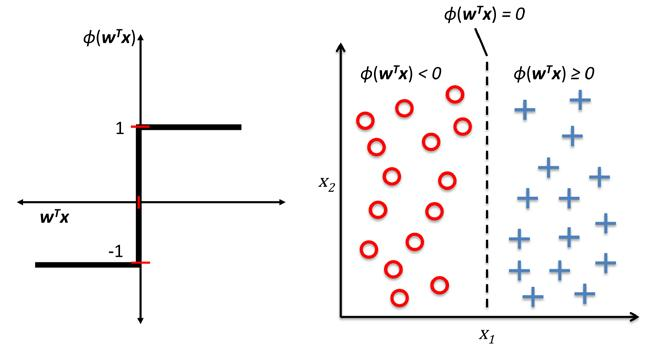
\includegraphics[scale=0.5]{perceptron}

La idea detrás del modelo de perceptron de Rosenblatt es la abstracción de cómo funciona
una neurona: se activa o no se activa. Así, la regla inicial de 

\end{document}
